\section{Aplicaciones}

Ejemplos por campos de aplicación:

\begin{itemize}
  \item Medicina \begin{itemize}
    \item Extracción de información a partir de imágenes médicas para el descubrimiento o tratamiento de enfermedades.
    \item Realzado de imágenes ruidosas para su interpretación por humanos.
    \item En robot terapéuticos, detección de caras y poses, clasificación de emociones, localización de puntos de mira.
  \end{itemize}
  \item Robótica \begin{itemize}
    \item Ayuda a la maquinaria en la fabricación, mediante inspección de los productos o la localización de elementos utilizados en una cadena de montaje.
    \item Para la navegación y el esquivo de obstáculos.
  \end{itemize}
  \item Seguridad \begin{itemize}
    \item Reconocimiento de personas mediante huellas dactilares.
    \item Identificación de caras.
    \item Detección de armas, video vigilancia.
  \end{itemize}
  \item Gráficos \begin{itemize}
    \item Reconstrucción de espacios 3D.
    \item Match moving: Juntar CGI con imágenes reales.
    \item Captura de formas y movimientos para efectos especiales.
  \end{itemize}
  \item Otros \begin{itemize}
    \item Soporte al cumplimiento de reglas en deportes.
    \item Modelado de terrenos y creación de imágenes panorámicas en misiones espaciales.
    \item Identificación forense.
    \item En el campo militar, guiado de misiles.
  \end{itemize}
\end{itemize}


\begin{figure}
  \centering  
  \begin{subfigure}[t]{0.48\textwidth}
    \centering
    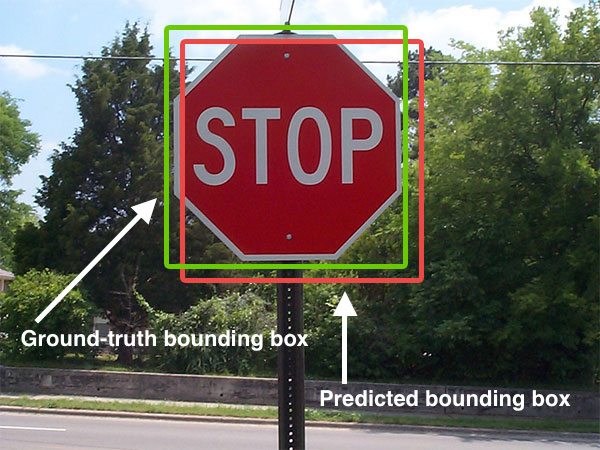
\includegraphics[width=\textwidth]{img/9.jpg}
  \end{subfigure}
  \vspace{7mm}
  \hfill
  \begin{subfigure}[t]{0.48\textwidth}
    \centering
    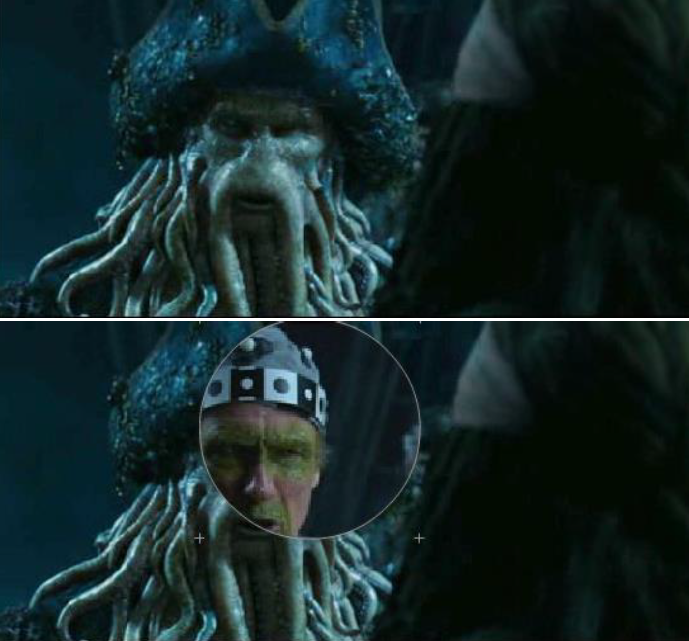
\includegraphics[width=\textwidth]{img/2.png}
  \end{subfigure}
  \hfill
  \begin{subfigure}[t]{0.48\textwidth}
    \centering
    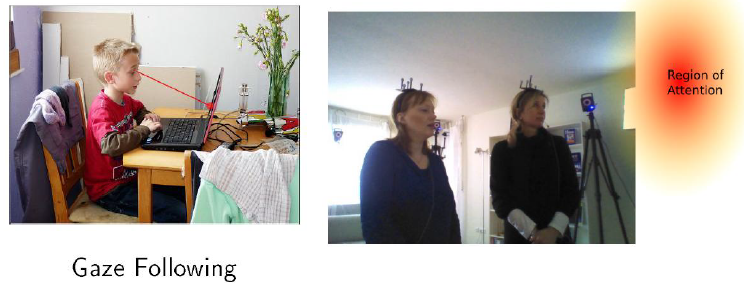
\includegraphics[width=\textwidth]{img/7.png}
  \end{subfigure}
  \hfill
  \begin{subfigure}[t]{0.48\textwidth}
    \centering
    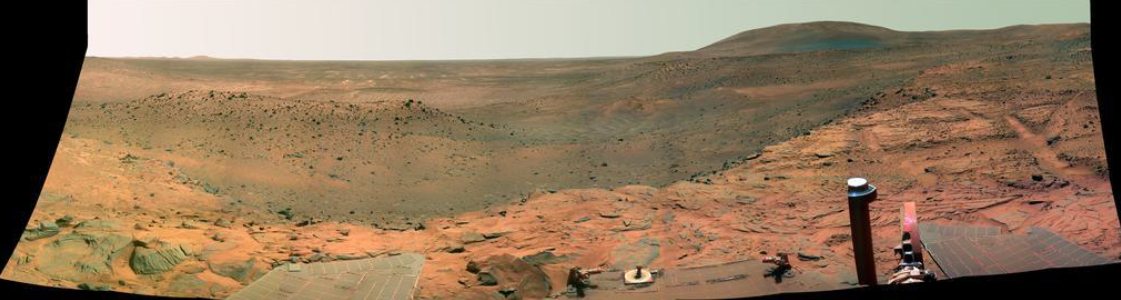
\includegraphics[width=\textwidth]{img/4.png}
  \end{subfigure}
  \hfill
  \begin{subfigure}[t]{0.48\textwidth}
    \centering
    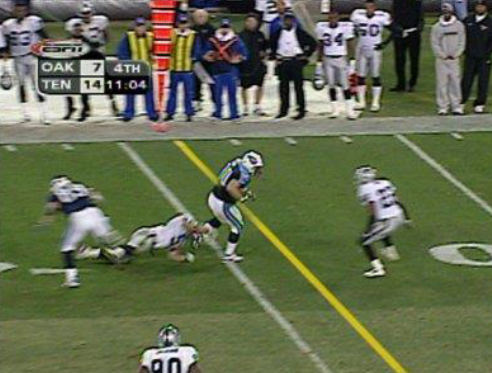
\includegraphics[width=\textwidth]{img/3.png}
  \end{subfigure}
  \hfill
  \begin{subfigure}[t]{0.48\textwidth}
    \centering
    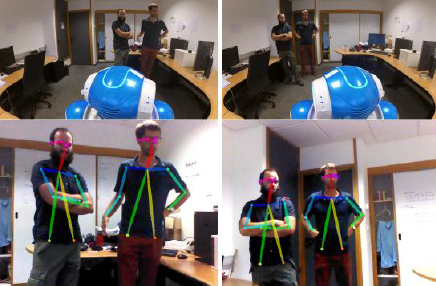
\includegraphics[width=\textwidth]{img/6.png}
  \end{subfigure}
  \hfill
  \begin{subfigure}[t]{0.48\textwidth}
    \centering
    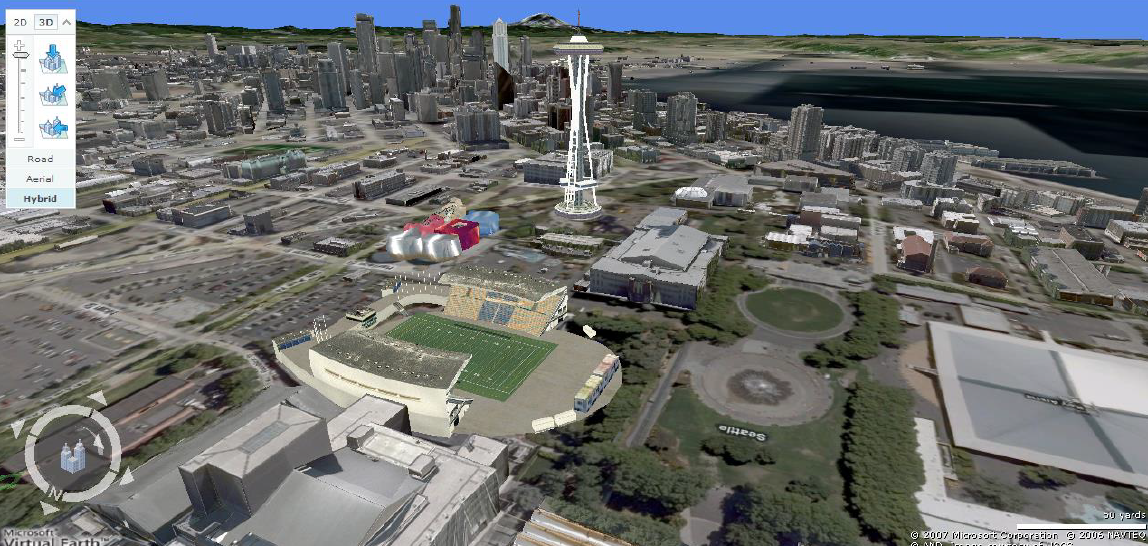
\includegraphics[width=\textwidth]{img/1.png}
  \end{subfigure}
  \hfill
  \begin{subfigure}[t]{0.48\textwidth}
    \centering
    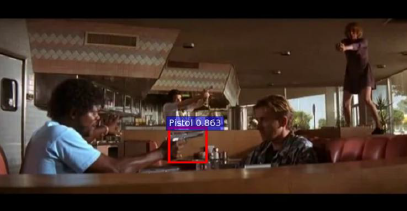
\includegraphics[width=\textwidth]{img/8.png}
  \end{subfigure}
  \hfill
  \begin{subfigure}[t]{0.48\textwidth}
    \centering
    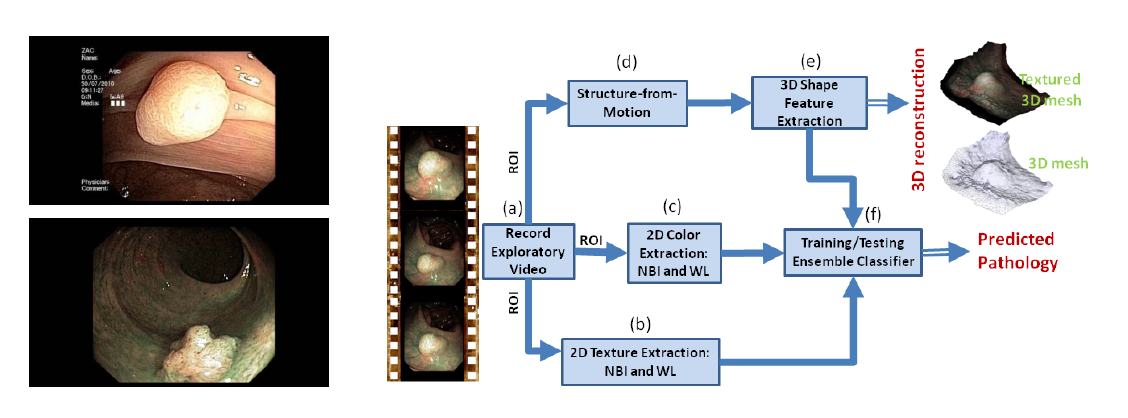
\includegraphics[width=\textwidth]{img/5.png}
  \end{subfigure}

  \caption{Aplicaciones de la visión artificial.}
\end{figure}

